For doing clustering for our data, we have looked at Gaussian Mixture Model and Hierarchical Clustering. For the Gaussian Mixture Modelling, we have used cross validation in order to determine the number of clusters that should be used for our problem.

%\subsection{Gaussian Mixture Model}

\subsection{Cross Validation}

We have performed cross validation in order to find the number of clusters that is most optimal for our data set. We have used 5-fold cross-validation, which will result in a test set of size 92 data objects and training set of size 370 data objects. We have set that the range of $K$, meaning the number of clusters, we look at range from 1-20. For each of these values of $K$, we create 5 different training and test sets to evaluate for. For each time, we create a Gaussian Mixture Model, we set the number repetitions to 10, meaning we try 10 different ways of setting placing the centroids randomly in our initial guess.

\begin{figure}[H]
\center
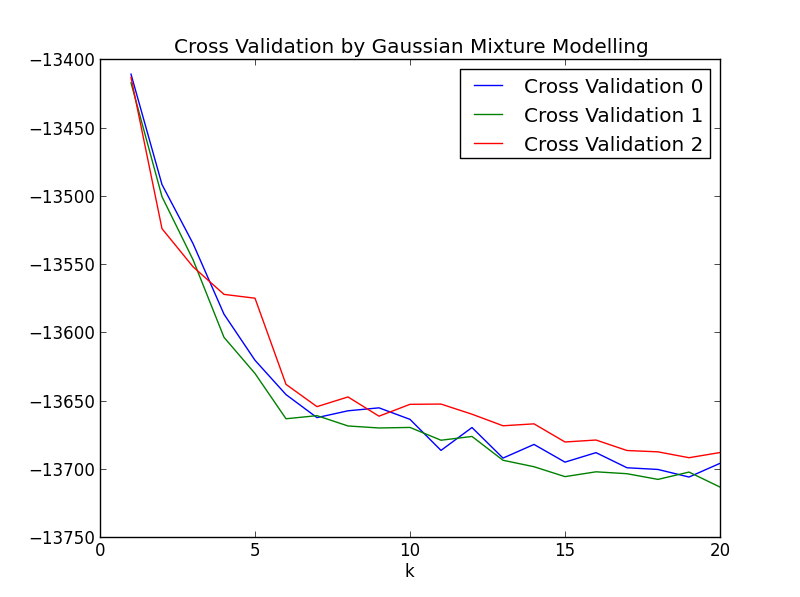
\includegraphics[scale=0.5]{pictures/CVKGaussian.png}
\caption{\footnotesize This shows the results of performing cross-validation on our data set according to find number of clusters.}
\label{CVK}
\end{figure}

In Figure \ref{CVK}, we plot the score of using different number of clusters. Generally, we see that the score gets better, when using more clusters. We see that the score gets better from using 1 to 6 clusters. After this the slope flattens.

\subsection{Gaussian Mixture Model}

For plotting the Gaussian Mixture Model, we have chosen to use 6 clusters, as this is where we see the most improvement according to Figure \ref{CVK}.

\begin{figure}[H]
\center
\hspace*{-1.5cm}
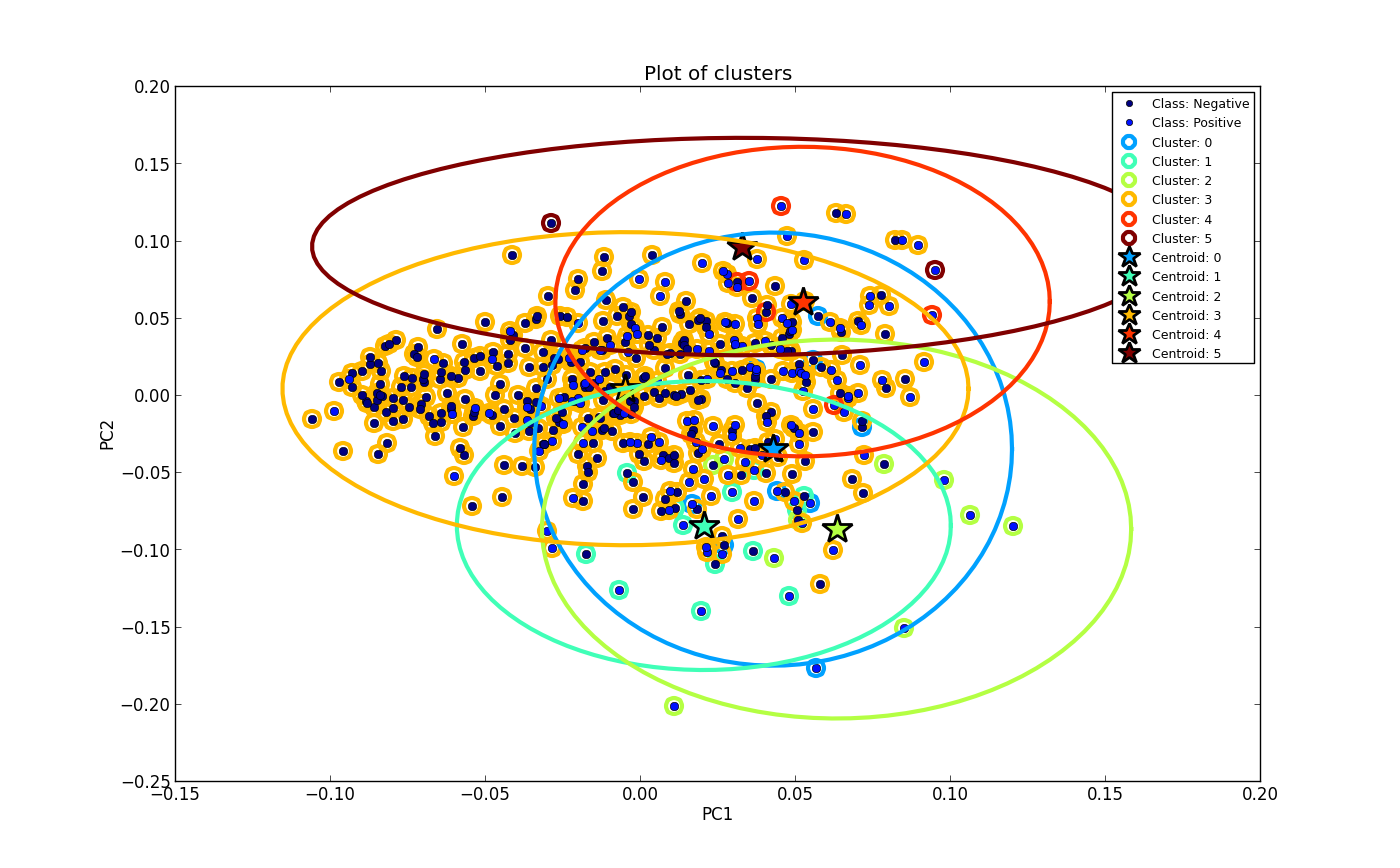
\includegraphics[scale=0.5]{pictures/GaussianK6.png}
\caption{\footnotesize This shows the data points plotted onto the two most describing principal component. For each point is shown whether the subject in fact has or does not have the disease. Furthermore it is shown which cluster the subject is assigned to.}
\label{GMM}
\end{figure}

In Figure \ref{GMM} we see our data points plotted according to which cluster, they are assigned. For doing this, we have converted our data, so that it is described by principal components. For doing our calculations, we have used all the data, and then we have plotted and shown the results projected onto the two most important principal components. We see that most of our data points have been assigned to cluster \MDC. In fact 422 of 462 data points are located in this cluster.

We see that most of our data points are located in the center, and that the density of points seems very high in the center. Most of these data points located in the center are assigned to cluster \MDC. But we also see that we have 5 small clusters. And especially the points located in the outer area of the plot are assigned to these clusters.

For most of our clusters, they both contain CHD-positive and CHD-negative members. In cluster \CN, we see that there is a high number of CHD-positive subjects compared to CHD-negative objects. In fact this cluster has 7 positive subjects and 3 negative subjects. So if a new data object would be assigned to this cluster, it could indicate a high probability of the subject being ill. For the other clusters it is harder to say anything useful about whether subjects would be CHD-positive or CHD-negative. For instance for cluster \MDC, we have 285 negative and 137 positive subjects. This means that roughly $\frac{1}{3}$ of the subjects in this cluster are CHD-positive, but is probably a result of that roughly $\frac{1}{3}$ of objects in the whole data set are CHD-positive.

%0.33

\subsection{Hierarchical Clustering}

We have done Hierarchical Clustering, where we have set the maximum number of clusters to be 6, as we did when using Gaussian Mixture Modelling. Furthermore, like we did for the Gaussian Mixture Model, we have projected the data onto principal components. We have used all the principal components, describing 100\% of the variance, to do the calculations, like calculating clusters and assigning clusters to data points. And then for plotting our results, we have projected the data onto the two most important principal components. This can lead to some clusters looking funny, as we can not see 100\% of the variance in the plot.

When doing hierarchical clustering, we have used euclidean distance measure. Furthermore, we have to choose a method, which is used to calculate the distance between two clusters. Examples of such methods are single, complete and average. Using single, when calculating the distance between two cluster, one chooses two nodes (one from each cluster), giving the smallest distance between the two clusters. For our example, this would result in a cluster holding practically all nodes, and then a few clusters holding a single node.  This is because the algorithm would start linking all the nodes located in the center of the plot, which are located close to each other. This way a cluster would grow from the center and then out, meaning in the end we would have a big cluster holding almost all the nodes, and then some clusters located in the outer range of the plot holding single nodes. Another approach is using the complete linkage method, where when we calculate the distance between two clusters, we look at the two nodes (one from each cluster), giving the biggest distance from each other. A third approach is to use the average method, where we calculate an average distance of the nodes in the two clusters. We look at all pairs of nodes (containing one node from each cluster), and calculate the average distance.

We will not look at the single linkage method, as this is not very describing for our data set, but in Figure \ref{HCResults}, one can see the results of doing hierarchical clustering using either the average or complete method.

\begin{figure}[H]
\begin{subfigure}[b]{1\textwidth}
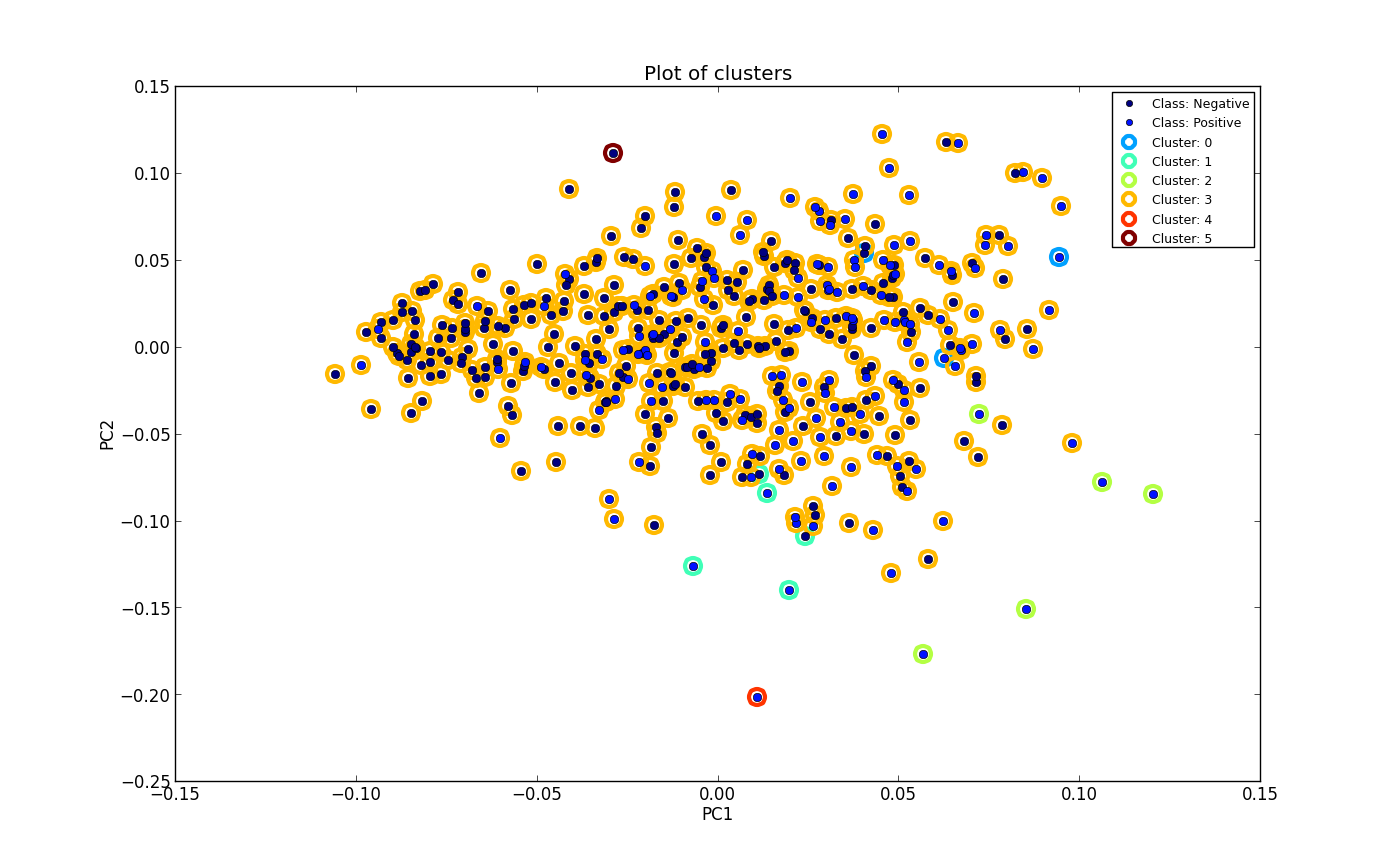
\includegraphics[scale=0.5]{pictures/HCAvg.png}
\caption{\footnotesize Hierarchical Clustering of data point using Average method.}
\label{HCResultsAVG}
\end{subfigure}
\begin{subfigure}[b]{1\textwidth}
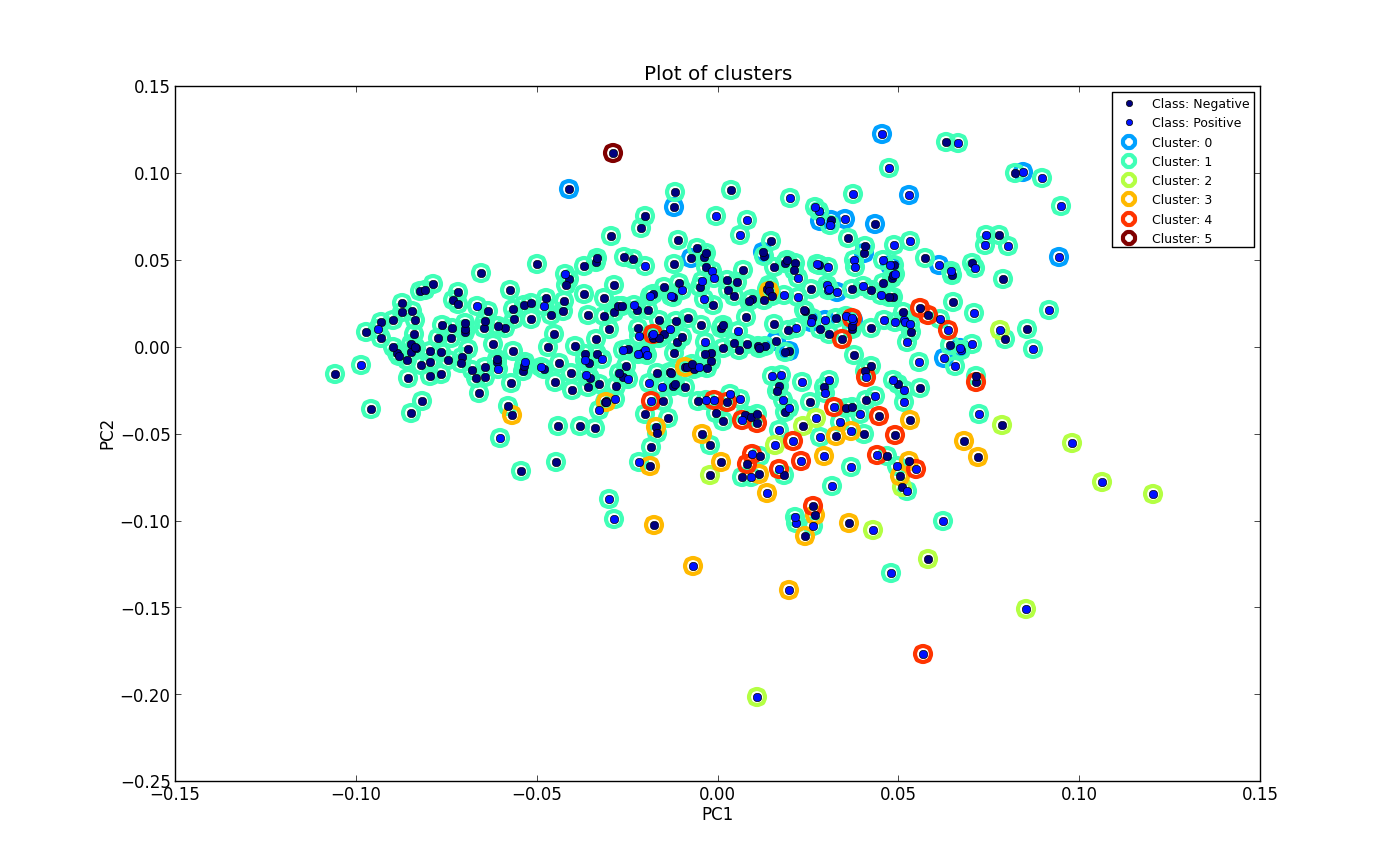
\includegraphics[scale=0.5]{pictures/HCCom.png}
\caption{\footnotesize Hierarchical Clustering of data points using Complete method.}
\label{HCResultsCOM}
\end{subfigure}
\caption{\footnotesize Hierarchical Clustering}
\label{HCResults}
\end{figure}

We see from Figure \ref{HCResults} that both when using the average and the complete method, we get a very big cluster containing the majority of the data points. For the average method, this is cluster \HCAVGD{} holding 447 data point, while for the complete method, it is cluster \HCCOMD{}  holding 375 elements.

Looking at Figure \ref{HCResultsCOM}, showing Hierarchical Clustering using the complete method, we see that for the clusters \HCCOMA{}, \HCCOMB{} and \HCCOMC{} that the majority of elements in these clusters are positive for the CHD-disease. In cluster \HCCOMA{} we have 15 positives compared to 10 negatives, in cluster \HCCOMB{} we have 9 positives compared to 5 negatives, and in cluster \HCCOMC{} we have 14 positives compared to 9 negatives. This could indicate that if a new data object is located in one of these clusters he is more likely to have the disease. Especially because the majority of subjects in the set are CHD-negative.

Furthermore in Figure \ref{dendrogram}, we can see how the nodes hierarchically are clustered together when using the complete method. We see that the object located furthest to the left on the x-axis is not linked to any other nodes until the last step. This means that this objects lies far away from all the other nodes. This object must correspond to the only node located in cluster \HCCOMS{} in Figure \ref{HCResultsCOM} as this cluster is the only one to have only one object.

\begin{figure}[H]
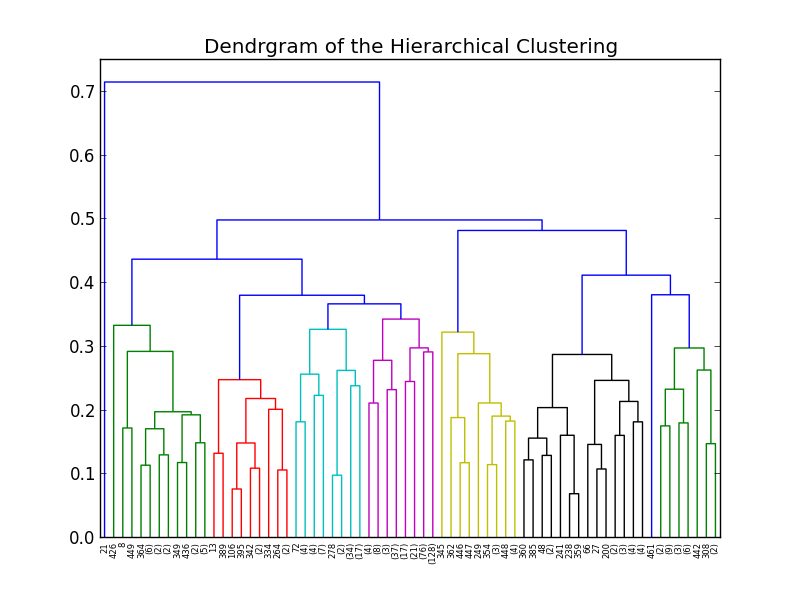
\includegraphics[scale=0.5]{pictures/dendrogram.png}
\caption{\footnotesize Dendrogram showing how the nodes are clustered hierarchically together.}
\label{dendrogram}
\end{figure}


\subsection{Evaluation}

As we can see, we can cluster our data objects into different clusters. However our data is not very well-suited for clustering, as in most cases, the majority of all points are located in the same cluster. This happens both when doing clustering using Gaussian Mixture Modelling and doing Hierarchical Clustering. However for both cases, we also see that we can model some clusters, where the majority of the data points are CHD-positive. This can be interesting, as this might indicate that subjects located in such clusters might have a higher possibility of being CHD-positive.